	\section*{Exercice 1 (5 points)}
	
	\subsection*{Question 1}
	
	
	On peut dresser un arbre pondéré de probabilités :
	
\begin{center}
	\pstree[treemode=R,nodesepA=0pt,nodesepB=3pt]{\TR{}}
	{\pstree{\TR{$A~~$} \naput{0,2}}
		{\TR{$C~~$}\naput{0,6}
			\TR{$\overline{C}~~$}\nbput{0,4}
		}
		\pstree{\TR{$\overline{A}~~$} \nbput{0,8}}
		{\TR{$C~~$}\naput{$x$}
			\TR{$\overline{C}~~$}\nbput{$1 - x$}
		}
	}
\end{center}
	
	On en déduit le tableau de la loi de $G$ :
	
	\[
	\begin{array}{|c|c|c|c|c|}
	\hline
		\text{Gain (G)} & -5 & 2 & 2 & 4 \\
		\hline
		\text{Probabilité} & \dfrac{1}{4} & \dfrac{1}{4} & \dfrac{1}{4} & \dfrac{1}{4} \\
		\hline
	\end{array}
	\]
	
	On a donc $$E(G) = \dfrac{1}{4} \times (-5) + \dfrac{1}{4} \times 2 + \dfrac{1}{4} \times 2 + \dfrac{1}{4} \times 4 = \dfrac{1}{4} \times (-5 + 2 + 2 + 4) = 3 \times \dfrac{1}{4} = \dfrac{3}{4} = 0,75$$
	
	La réponse correcte est \textbf{a.}
	
	\subsection*{Question 2}
	
	On sait que $P(A \cup B) = P(A) + P(B) - P(A \cap B)$, soit
	\[
	\dfrac{4}{7} = \dfrac{3}{7} + \dfrac{3}{20} - P(A \cap B)
	\]
	
	d’où :
	\[
	P(A \cap B) = \dfrac{3}{7} + \dfrac{3}{20} - \dfrac{4}{7} = \dfrac{3}{20} - \dfrac{1}{7} = \dfrac{21}{140} - \dfrac{20}{140} = \dfrac{1}{140}
	\]
	
\begin{itemize}
	\item 	$P(A)\times P(B) = \dfrac{9}{140}$ et 	$P(A \cap B) = \dfrac{1}{140}$ donc les évènements A et B ne sont donc pas indépendants.
	
\item	$
	P_A(B) = \dfrac{P(A \cap B)}{P(A)} = \dfrac{1}{140} \div \dfrac{3}{7} = \dfrac{1}{140} \times \dfrac{7}{3} = \dfrac{1}{60}
$
	
\item 	$P(A \cap B) = \dfrac{1}{140}$
	\end{itemize}
	
	Il y a deux bonnes réponses !!
	\subsection*{Question 3}
	
	D’après la loi des probabilités totales :
	\[
	P(C) = P(A \cap C) + P(\overline{A} \cap C) = 0,2 \times 0,6 + 0,8 \times x = 0,48
	\]
	
	Donc
	\[
	0,12 + 0,8x = 0,48 \quad \text{ou} \quad 0,8x = 0,36 \quad \text{puis} \quad 80x = 36 \quad \text{et enfin} \quad x = \dfrac{36}{80} = \dfrac{9}{20} = 0,45
	\]
	
	La réponse correcte est \textbf{c.}
	
	\subsection*{Question 4}
	

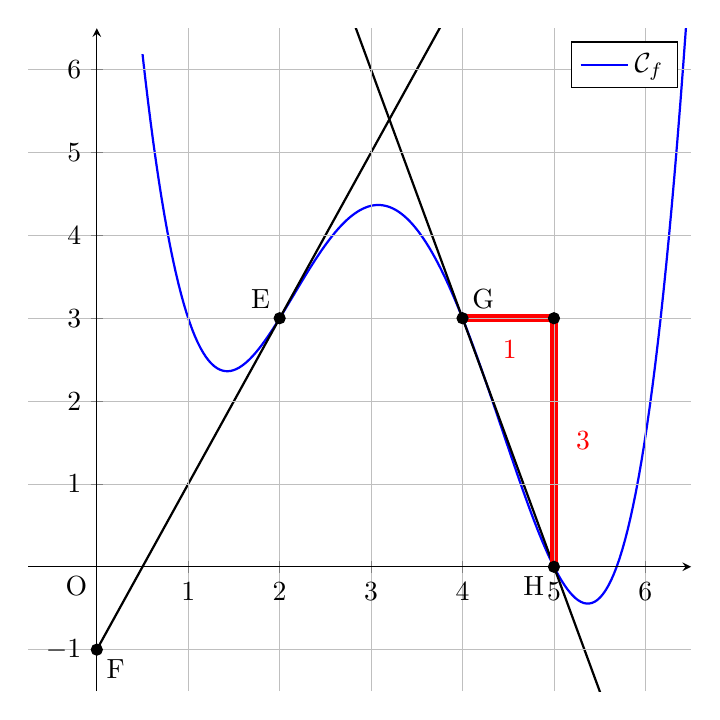
\begin{tikzpicture}
	\begin{axis}[
		axis lines=middle,
		xmin=-0.75, xmax=6.5,
		ymin=-1.5, ymax=6.5,
		xtick={0,1,2,3,4,5,6},
		ytick={-1,0,1,2,3,4,5,6},
		grid=both,
		grid style={line width=.1pt, draw=gray!10},
		major grid style={line width=.2pt,draw=gray!50},
		width=10cm,
		height=10cm,
		axis on top,
		samples=200
		]
		
		% Plotting the functions
		\addplot [
		domain=0.5:6.5,
		samples=200,
		thick,
		blue
		]
		{(x - 5) * ((3 * x^3 / 14) - (1.75 * x^2) + (3.5 * x) - (19 / 7))};
		\addlegendentry{$\mathcal{C}_f$}
		
		\addplot [
		domain=0:4,
		samples=200,
		thick
		]
		{2 * x - 1};
		
		\addplot [
		domain=2.5:6,
		samples=200,
		thick
		]
		{15 - 3 * x};
		
		% Adding points
		\addplot[only marks, mark=*] coordinates {(0,-1) (2,3) (4,3) (5,0) (5,3)};
		\node[below right] at (axis cs:0,-1) {F};
		\node[above left] at (axis cs:2,3) {E};
		\node[above right] at (axis cs:4,3) {G};
		\node[below left] at (axis cs:5,0) {H};
		\node[below left] at (axis cs:0,0) {O};
		
		% Adding red segment
		\addplot[red, line width=3pt] coordinates {(5,0) (5,3)};
			\addplot[red, line width=3pt] coordinates {(4,3) (5,3)};
				\node[below left,red] at (axis cs:4.7,2.85) {$1$};
					\node[below left,red] at (axis cs:5.5,1.75) {$3$};
		
	\end{axis}
\end{tikzpicture}

	La pente de la tangente au point $G$ est -3, donc $f'(4) = -3$.
	
	La réponse correcte est \textbf{d.}
	
	\subsection*{Question 5}
	
\texttt{evolu(500) = 4}
	
	La réponse correcte est \textbf{a.}
	
